% =====================================================================
%  VeriCloud final report -- main file
%  OWNER: A (Zuo Yuhong). Nobody else edits this file or the preamble.
%  Everyone else writes only in their own sections/*.tex file.
%  Layout follows the team's Word proposal: Times New Roman 12pt,
%  Lingnan logo cover, "Section n:" headings, dotted Table of Contents.
% =====================================================================
\documentclass[12pt,a4paper]{article}

% ---------- cover information: A edits these lines only ----------
\newcommand{\reportkind}{Final Report}
\newcommand{\presentationdate}{Nov.24,2026}
\newcommand{\submissiondate}{TBD}        % TODO(A): fill in once the deadline is confirmed

% ---------- page layout (same margins as the Word proposal) ----------
\usepackage[a4paper, top=2.54cm, bottom=2.54cm, left=3.17cm, right=3.17cm,
            headheight=15pt, headsep=0.9cm, footskip=1.2cm]{geometry}
\usepackage{newtxtext,newtxmath}         % Times New Roman look
\usepackage{graphicx}
\usepackage{booktabs}
\usepackage{array}
\usepackage{caption}
\usepackage{amsmath}
\usepackage{listings}
\usepackage{xcolor}
\usepackage{setspace}
\usepackage{fancyhdr}
\usepackage{titlesec}
\usepackage{tocloft}

% ---------- header / footer: small course name top right, page number bottom centre ----------
\pagestyle{fancy}
\fancyhf{}
\fancyhead[R]{\scriptsize CDS538 Cloud Computing}
\fancyfoot[C]{\footnotesize\thepage}
\renewcommand{\headrulewidth}{0pt}
\renewcommand{\footrulewidth}{0pt}
\fancypagestyle{plain}{\fancyhf{}\fancyhead[R]{\scriptsize CDS538 Cloud Computing}%
  \fancyfoot[C]{\footnotesize\thepage}\renewcommand{\headrulewidth}{0pt}}

% ---------- body headings: "Section 1: Title" 16pt bold, subsections 12pt bold ----------
\titleformat{\section}{\fontsize{16}{20}\selectfont\bfseries}{Section \thesection:}{0.4em}{}
\titleformat{\subsection}{\normalsize\bfseries}{\thesubsection}{0.6em}{}
\titleformat{\subsubsection}{\normalsize\bfseries}{\thesubsubsection}{0.6em}{}
\titlespacing*{\section}{0pt}{18pt}{10pt}
\titlespacing*{\subsection}{0pt}{12pt}{6pt}
\titlespacing*{\subsubsection}{0pt}{10pt}{4pt}

% ---------- Table of Contents: same look as the Word proposal ----------
\renewcommand{\contentsname}{Table of Contents}
\renewcommand{\cfttoctitlefont}{\fontsize{16}{20}\selectfont\bfseries}
\setlength{\cftbeforetoctitleskip}{0pt}
\setlength{\cftaftertoctitleskip}{14pt}
\renewcommand{\cftdotsep}{1}                         % dense dots like Word
% level 1: "Section 1: Title ........ 2", not bold
\renewcommand{\cftsecfont}{\normalfont}
\renewcommand{\cftsecpagefont}{\normalfont}
\renewcommand{\cftsecleader}{\cftdotfill{\cftdotsep}}
\renewcommand{\cftsecpresnum}{Section~}
\renewcommand{\cftsecaftersnum}{:}
\setlength{\cftsecnumwidth}{4.75em}
\cftsetpnumwidth{1.2em}                              % dots run close to the page number
\cftsetrmarg{1.8em}
\setlength{\cftsecindent}{0pt}
\setlength{\cftbeforesecskip}{0pt}
% level 2: indented "1.1 Title ........ 2"
\setlength{\cftsubsecindent}{2em}
\setlength{\cftsubsecnumwidth}{2.2em}
% level 3: indented further
\setlength{\cftsubsubsecindent}{4.2em}
\setlength{\cftsubsubsecnumwidth}{3em}
\setcounter{tocdepth}{3}

% ---------- code listings ----------
\lstdefinelanguage{json}{basicstyle=\ttfamily\small, showstringspaces=false,
  string=[s]{"}{"}, stringstyle=\color{blue!60!black}}
\lstset{basicstyle=\ttfamily\small, breaklines=true, frame=single, columns=fullflexible}

\usepackage[hidelinks]{hyperref}                     % load last

\begin{document}

% =====================================================================
%  COVER (no header, no page number)
% =====================================================================
\begin{titlepage}
  \hypersetup{pageanchor=false}                      % cover has no page number
  \centering
  \vspace*{-0.4cm}
  
\includegraphics[width=\textwidth]{figures/lingnan_logo.jpg}\par
  \vspace{2.8cm}
  {\fontsize{24}{30}\selectfont\bfseries CLOUD COMPUTING\par}
  \vspace{16pt}
  {\fontsize{24}{30}\selectfont\bfseries \reportkind\par}
  \vspace{3cm}
  {\renewcommand{\arraystretch}{1.75}%
  \begin{tabular}{@{}>{\bfseries\raggedleft\arraybackslash}p{3.6cm}@{\hspace{0.35cm}}>{\centering\arraybackslash}p{6cm}@{}}
    Course :            & CDS538 \\ \cline{2-2}
    Team name :         & SkyFin \\ \cline{2-2}
    Member :            & 5561009 ZUO YUHONG \\ \cline{2-2}
                        & 5538856 SU CHANGWEI \\ \cline{2-2}
                        & 5552072 YANG XUELI \\ \cline{2-2}
                        & 5546554 LI DONGHAN \\ \cline{2-2}
                        & 5520483 LI HENGCHEN \\ \cline{2-2}
                        & 3162304 HU ZHONGYUAN \\ \cline{2-2}
    Presentation date:  & \presentationdate \\ \cline{2-2}
    Submission date:    & \submissiondate \\ \cline{2-2}
    GitHub :            & {\small github.com/zuoyuhong783-sudo/KYC} \\ \cline{2-2}
  \end{tabular}\par}
\end{titlepage}

% =====================================================================
%  TABLE OF CONTENTS (page 1, like the Word proposal)
% =====================================================================
\hypersetup{pageanchor=true}
\setcounter{page}{1}
\begingroup
  \setstretch{1.75}
  \tableofcontents
\endgroup
\clearpage

% =====================================================================
%  ABSTRACT
% =====================================================================
\section*{Abstract}
\addcontentsline{toc}{section}{Abstract}
% TODO(A): write the abstract (E and F provide one result sentence each).

\noindent\textbf{Keywords:} serverless, KYC, AWS Step Functions, fault tolerance, cloud economics
\clearpage

% =====================================================================
%  BODY -- one file per owner (see the Overleaf guide)
% =====================================================================
% =====================================================================
%  OWNER: A. Only A edits this file; others use Overleaf comments.
%  Content: Background in one paragraph; objectives O1--O4 and how far each was achieved.
% =====================================================================
\section{Executive Summary and Project Objectives}\label{sec:summary}

% TODO(A): write this part.

% =====================================================================
%  OWNER: F. Only F edits this file; others use Overleaf comments.
%  Content: Industry pain points, cloud adoption motivation, KYC verification rules.
% =====================================================================
\section{Business Problem Framing and Requirements Analysis}\label{sec:business}

\subsection{Industry Background and Traditional Pain Points}\label{sec:business:background}

Customer onboarding is the first operational contact a bank has with a new
customer, and it is also the point at which regulatory risk and commercial
pressure collide. Under anti-money-laundering rules a bank must verify that an
applicant is who they claim to be before an account is opened: the identity
document has to be genuine and unexpired, and the person submitting it has to be
the person depicted on it. In a branch this is a manual task; in digital
onboarding it must be automated at scale, and the volume is strongly \emph{bursty}
because acquisition is driven by promotional campaigns rather than by a stable
daily arrival rate.

Traditional on-premises provisioning handles this burstiness badly, for three
reasons.

\begin{itemize}
  \item \textbf{Idle capacity versus over-provisioning.} Normal operating load
        typically consumes a small fraction of the provisioned server capacity,
        so most of the hardware is idle for most of the year. Provisioning
        additionally for the peak of a marketing campaign means paying for
        capital equipment that is used for a few days at a time.
  \item \textbf{Latency blow-ups at the peak.} When a campaign lands, a fixed
        infrastructure saturates: verification jobs queue behind each other, the
        queueing delay dominates the end-to-end time, and applicants abandon the
        flow. Industry data cited in the project proposal puts application
        abandonment at roughly 10\% when onboarding latency grows.
  \item \textbf{CapEx and operational drag.} Servers, storage, licences and the
        staff who maintain them are committed before a single application
        arrives. Every capacity decision is a multi-month procurement decision,
        which is the opposite of what a two-week campaign requires.
\end{itemize}

These are not tuning problems; they follow from the shape of the workload. A
verification pipeline is idle most of the time and extremely busy for short
intervals, which is precisely the profile that fixed-capacity infrastructure
prices worst.

\subsection{Cloud Adoption Motivation and Economic Value}\label{sec:business:cloud}

Cloud computing addresses the capacity-versus-cost conflict through two of the
essential characteristics defined by NIST~\cite{mell2011nist}, both of which this
project relies on directly:

\begin{itemize}
  \item \textbf{Rapid elasticity.} Compute is allocated per request rather than
        pre-purchased. When a burst of applicants arrives, an equal number of
        serverless execution environments are created in parallel and released
        as soon as each verification finishes, so the queue does not accumulate
        and the peak does not have to be provisioned for in advance.
  \item \textbf{Measured service (CapEx to OpEx).} Billing follows actual
        invocation count, execution duration and bytes stored. In the idle
        periods between campaigns the compute charge is zero, which converts a
        fixed capital commitment into a variable operating expense that tracks
        revenue.
\end{itemize}

The architectural consequence is that the unit of deployment stops being a
server and becomes an event. VeriCloud is therefore designed as an event-driven,
serverless pipeline in which every stage scales independently, following the
serverless application guidance of the AWS Well-Architected
Framework~\cite{aws2022serverlesslens}. The economic consequence is quantified in
Section~\ref{sec:cost}.

\subsection{KYC Compliance and Verification Rules}\label{sec:business:rules}

Automation is only acceptable if it remains auditable. The pipeline therefore
enforces a small set of quantitative rules, evaluated in a fixed order, so that
every application receives exactly one reproducible verdict. Table~\ref{tab:rules}
states them.

\begin{table}[htbp]
  \centering
  \small
  \caption{KYC decision rules, evaluated in order (first match wins).}
  \label{tab:rules}
  \begin{tabular}{@{}clll@{}}
    \toprule
    \# & Condition & Verdict & Reason code \\
    \midrule
    1 & OCR could not extract the required fields & \texttt{FAIL} & \texttt{ocr\_failed} \\
    2 & Document expired (\texttt{id\_valid = false}) & \texttt{FAIL} & \texttt{id\_expired} \\
    3 & Face comparison raised an error & \texttt{NEEDS\_HUMAN\_REVIEW} & \texttt{face\_error} \\
    4 & Similarity below the 80\% threshold & \texttt{NEEDS\_HUMAN\_REVIEW} & \texttt{similarity\_below\_80} \\
    5 & None of the above & \texttt{PASS} & \texttt{auto\_approved} \\
    \bottomrule
  \end{tabular}
\end{table}

Three design choices in Table~\ref{tab:rules} deserve comment. First, the rules
are \emph{ordered}: a missing extraction must never fall through to an approval,
and an expired document fails regardless of how well the faces match. Second, the
80\% similarity threshold is the only tunable in the automated path; it
is deliberately conservative, because the cost of a false acceptance in KYC is
far higher than the cost of a manual review. Third, anything that cannot be
decided automatically is routed to \texttt{NEEDS\_HUMAN\_REVIEW} rather than
being rejected, and the successfully extracted document fields are retained so
that the compliance officer does not have to re-key them. The system degrades to
a human, not to an error.

Files that are corrupt, empty or of an unsupported format are handled even
earlier: they fail validation before the workflow starts, are retried three
times, and are then quarantined in a dead-letter queue for 14 days. Such
applications never reach the decision table and never create a record, which
keeps the audit table free of unverifiable submissions.


\section{Target Cloud Architecture and Workflow Design}\label{sec:arch}
% =====================================================================
%  OWNER: A. Only A edits this file; others use Overleaf comments.
%  Content: Architecture figure (figures/fig_a_architecture.pdf) and the end-to-end data flow.
%  Figure source: GitHub docs/vericloud_architecture.drawio (open in draw.io to edit).
% =====================================================================
\subsection{Architectural Overview and System Flow}\label{sec:overview}

% TODO(A): write the overview text (task A7). Walk through steps 1-7 shown in Fig.~\ref{fig:architecture}.

% The diagram is very wide, so it gets its own rotated (landscape) page.
\begin{sidewaysfigure}
  \centering
  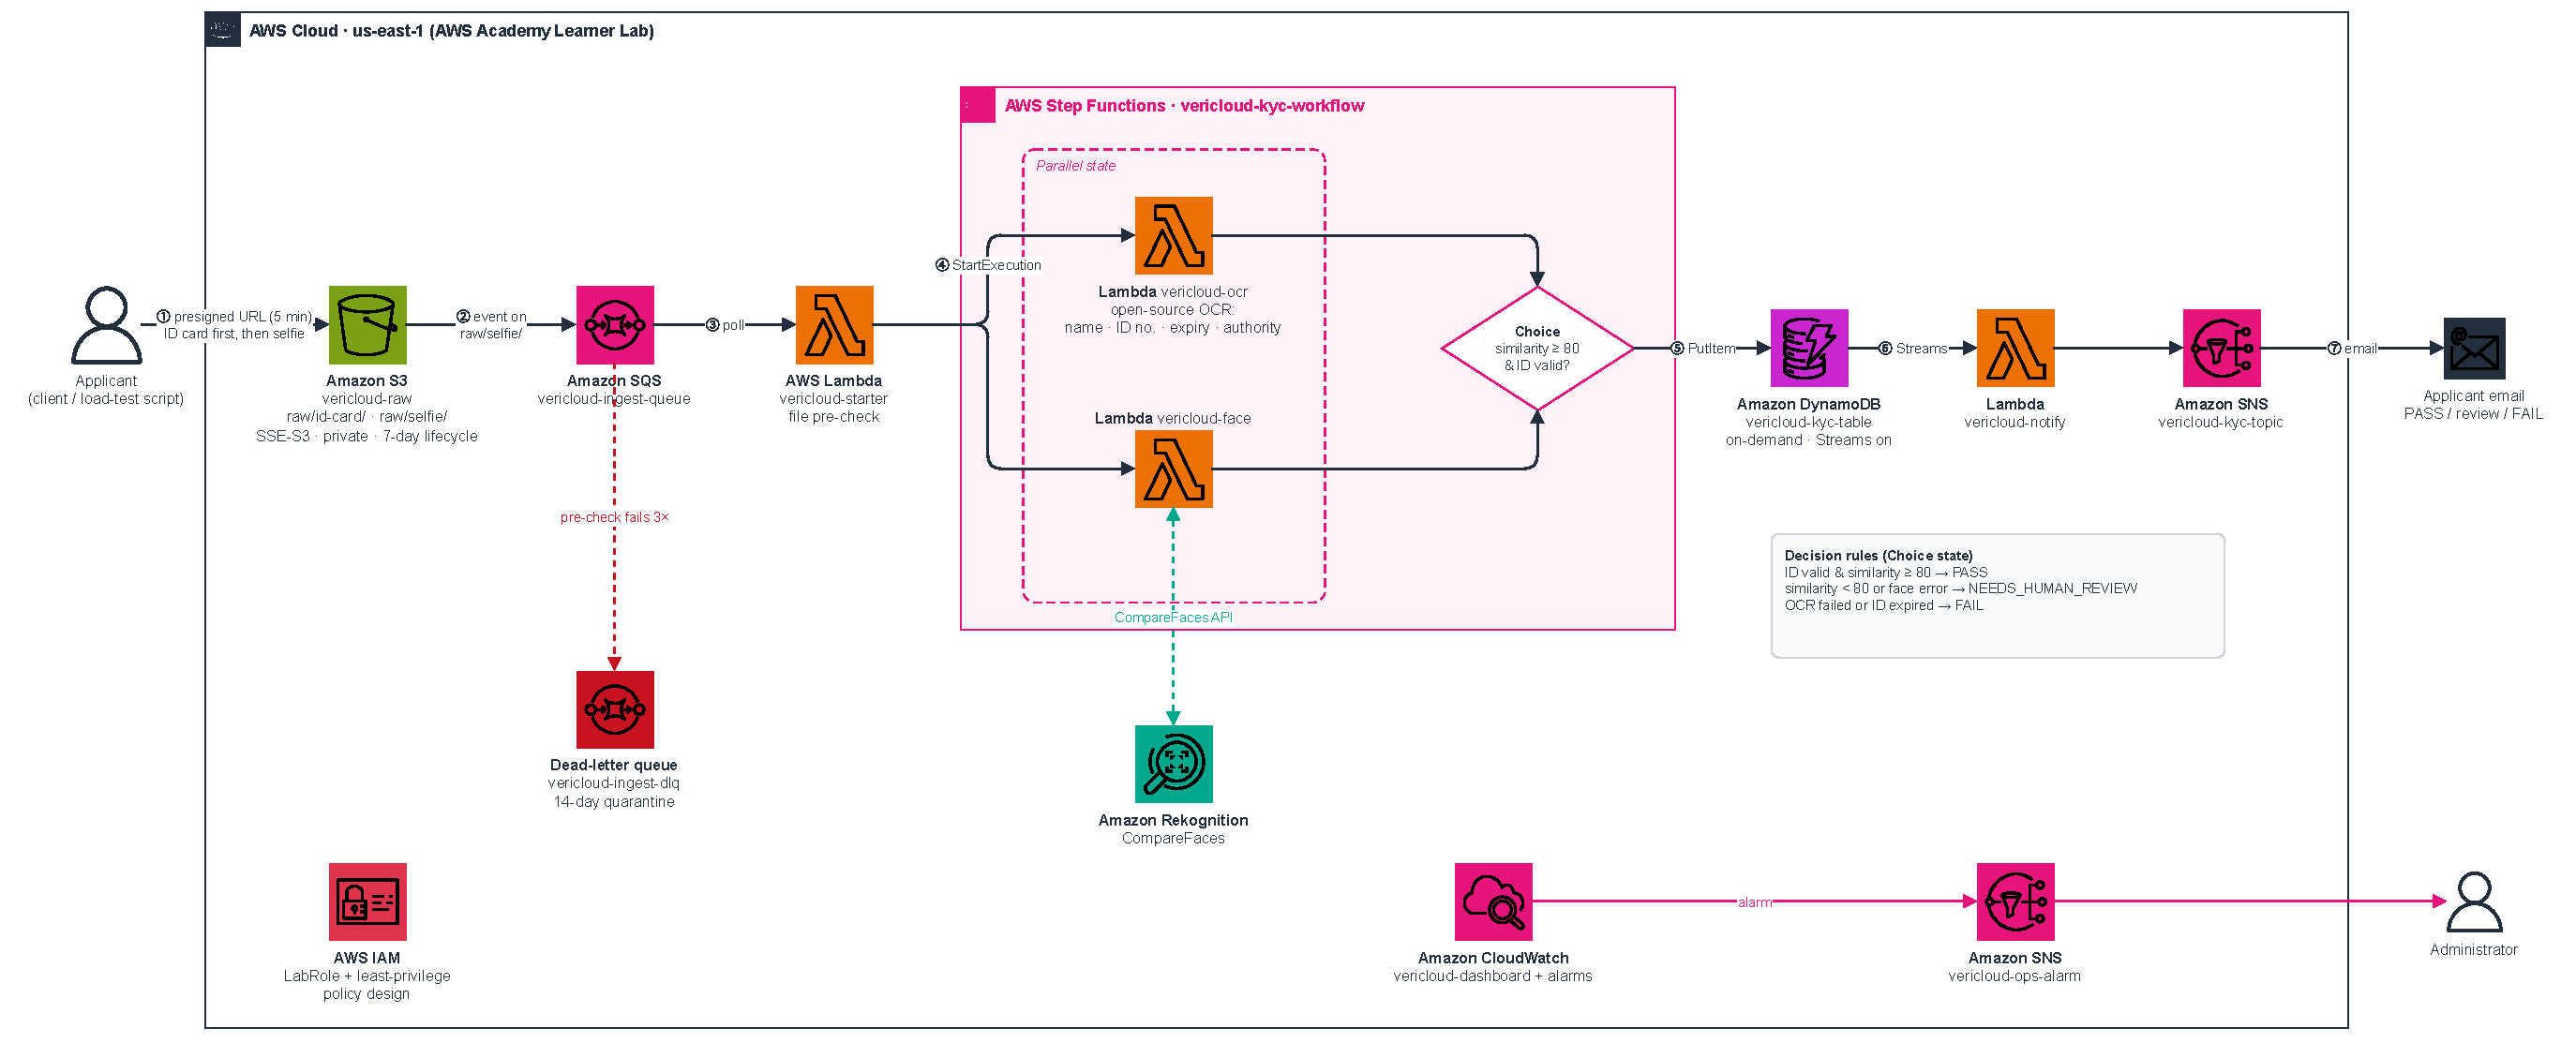
\includegraphics[width=\linewidth]{figures/fig_a_architecture.pdf}
  \caption{Architectural topology of the VeriCloud serverless KYC pipeline.}
  \label{fig:architecture}
\end{sidewaysfigure}

% =====================================================================
%  OWNER: D. Only D edits this file; others use Overleaf comments.
%  Content: State machine figure; Parallel, Retry/Catch, Choice and DynamoDB PutItem.
% =====================================================================
\subsection{Serverless Workflow Orchestration}\label{sec:orchestration}

% TODO(D): write this part.

\subsection{Core Processing Modules}\label{sec:modules}
% =====================================================================
%  OWNER: B. Only B edits this file; others use Overleaf comments.
%  Content: Library selection, packaging as a container image, field extraction, accuracy table, limitations.
% =====================================================================
\subsubsection{OCR Text Extraction Module}\label{sec:ocr}

% TODO(B): write this part.

% =====================================================================
%  OWNER: C. Only C edits this file; others use Overleaf comments.
%  Content: Amazon Rekognition CompareFaces, the 80\% threshold, error handling.
% =====================================================================
\subsubsection{Face Verification Module}\label{sec:face}

% TODO(C): write this part.

% =====================================================================
%  OWNER: F. Only F edits this file; others use Overleaf comments.
%  Content: DynamoDB schema, Streams, the notify Lambda and SNS email.
% =====================================================================
\subsubsection{Data Schema and Notification}\label{sec:data}

% TODO(F): write this part.


% =====================================================================
%  OWNER: D. Only D edits this file; others use Overleaf comments.
%  Content: SQS dead-letter queue, Retry/Catch, graceful degradation to human review.
% =====================================================================
\section{System Exception Handling and Fault Tolerance Design}\label{sec:fault}

% TODO(D): write this part.


\section{Security, Compliance and Cost Optimization}\label{sec:seccost}
% =====================================================================
%  OWNER: C. Only C edits this file; others use Overleaf comments.
%  Content: Presigned URLs, SSE-S3, least-privilege IAM design, data minimisation, lifecycle rules.
% =====================================================================
\subsection{Security Architecture and Compliance Governance}\label{sec:security}

% TODO(C): write this part.

% =====================================================================
%  OWNER: F. Only F edits this file; others use Overleaf comments.
%  Content: Pricing Calculator comparison, measured cost from the load test, savings percentage.
% =====================================================================
\subsection{Total Cost of Ownership and Cloud Economics}\label{sec:cost}

% TODO(F): write this part.


% ============================================================
%  sec6_testing.tex —— Ch6 Performance Testing and Monitoring
%  负责人：Li Hengchen (E)
%  粘贴到 Overleaf 的 sections/sec6_testing.tex
%
%  写作约定（《02_Overleaf 指南》）：
%   · 本节用 \section 起头（main.tex 不再包一层）
%   · 只写正文，不要 \documentclass / \begin{document}
%   · 数字必须来自 results/*.csv，禁止手抄、禁止估
%   · 图：文件放 report/figures/，LaTeX 里仍写 figures/xxx（相对 report/main.tex 解析）
%   · 表：tables/tab_e_loadtest.tex（由 collect_results.py --latex 生成）
%   · 特殊字符：\% $\geq$ $\times$，下划线用 \_
%
%  待 A 审核的跨人引用：
%   · \ref{sec:fault} 指向 D 的 Ch4（sec4_fault_tolerance.tex）
%   · \cite{aws2023security} 已在 references.bib；\cite{aws2024cloudwatch}
%     需 F 追加（条目见 docs/e_bib_entries.bib）
% ============================================================

\section{Performance Testing and Monitoring}\label{sec:testing}

Functional correctness alone does not establish that an onboarding pipeline is
usable: a KYC service must also absorb a traffic burst without dropping valid
applications and must isolate malformed uploads without stalling the queue. This
section defines the metrics that were instrumented, describes the fault-injected
workload and the fixture suite behind it, explains how alarms convert those
measurements into an operational response, and states the limits of what the
measurements can support.

\subsection{Observability Metrics and Instrumentation}\label{sec:metrics}

A single CloudWatch dashboard (\texttt{vericloud-dashboard}) consolidates four
families of metrics; the choice follows the operational-visibility guidance of
the AWS Well-Architected Framework~\cite{aws2023security}, while the alarm
thresholds are derived from the failure taxonomy in
Section~\ref{sec:fault}~\cite{aws2024cloudwatch}:

\begin{itemize}
  \item \textbf{Invocations and concurrency} per worker Lambda, to show that
        concurrency scales with the burst and returns to zero once the queue
        drains;
  \item \textbf{Duration} reported at p90 and p99 rather than the mean, because
        the mean hides the cold-start tail that users actually perceive;
  \item \textbf{Errors and throttles} across Lambda, DynamoDB and Step
        Functions, which distinguish application faults from capacity limits;
  \item \textbf{Queue depth} (\texttt{ApproximateNumberOfMessagesVisible}) for
        both the ingestion queue and the dead-letter queue, the leading
        indicator of back-pressure.
\end{itemize}

Latency is reported under three explicit clocks, because a single number hides
where the time is spent. \emph{Ingress latency} runs from the completion of the
client upload (\texttt{created\_at}, the S3 \texttt{eventTime}) to the moment
the pre-check Lambda starts (\texttt{received\_at}), and therefore covers event
delivery, queueing and the cold start of the first function. \emph{Service
latency} runs from \texttt{received\_at} to \texttt{processed\_at} and covers
only pipeline work. \emph{End-to-end latency} runs from the client-side
completion of the selfie upload (\texttt{t\_submit\_utc}) to
\texttt{processed\_at}, and is the number a user would experience. Separating
the three prevents the common mistake of quoting a service-internal figure as the
user-visible response time.

Percentiles are preferred to the arithmetic mean for a second reason: the
distribution of end-to-end latency in an event-driven pipeline is right-skewed,
because a small number of requests either hit a cold start or wait behind a
queue. A mean would average those cases into an unremarkable number, whereas p90
and p99 keep them visible.

\subsection{Workload Design and Fault Injection}\label{sec:workload}

The load generator dispatches 100 application packages within a 60-second
window, roughly 1.7 requests per second. In the default \emph{uniform} profile
packages are paced evenly, which measures sustained throughput without allowing
a queue to build up; a separate \emph{burst} profile releases the same 100
packages within ten seconds to observe concurrency ramp-up and cold-start
behaviour. Each package consists of one identity-document image and one selfie,
uploaded through 5-minute presigned URLs in that order; the selfie upload is the
event that triggers the workflow.

Twenty percent of the packages are deliberately corrupted (zero-byte files,
non-image payloads renamed to \texttt{.jpg}, and truncated JPEG streams), mixed
uniformly into the whole submission window rather than front-loaded, so that the
dead-letter path is exercised concurrently with the happy path. A separate
functional suite of 27 fixtures covers all four verdicts---\texttt{PASS},
\texttt{NEEDS\_HUMAN\_REVIEW}, \texttt{FAIL} and \texttt{DLQ}---as
summarised in Table~\ref{tab:fixtures}.

\begin{table}[htbp]
  \centering
  \small
  \caption{Functional fixture coverage by expected verdict.}
  \label{tab:fixtures}
  \begin{tabular}{llc}
    \toprule
    Category & Expected outcome & Cases \\
    \midrule
    Normal (same person, valid document) & \texttt{PASS} & 10 \\
    Identity mismatch & \texttt{NEEDS\_HUMAN\_REVIEW} & 3 \\
    Blurred selfie & \texttt{NEEDS\_HUMAN\_REVIEW} & 2 \\
    Face-less selfie & \texttt{NEEDS\_HUMAN\_REVIEW} & 2 \\
    Expired document & \texttt{FAIL} & 2 \\
    Missing OCR field & \texttt{FAIL} & 2 \\
    Zero-byte upload & DLQ & 2 \\
    Wrong format / truncated & DLQ & 4 \\
    \midrule
    Total & & 27 \\
    \bottomrule
  \end{tabular}
\end{table}

The two blurred selfies deserve a note: a blurred capture may still expose a face
that simply fails the similarity threshold, or it may expose no usable face at
all. Both outcomes are correct for this category and both are classified as
\texttt{NEEDS\_HUMAN\_REVIEW}, so the expected reason for these two cases is
recorded as either \texttt{face\_error} or \texttt{similarity\_below\_80}.

The fixtures are generated locally and exchanged as a content-addressed bundle:
image files are kept out of the repository for privacy, and a SHA-256 manifest
allows every team member to confirm that they are testing against byte-identical
inputs. Without that check, three copies generated independently on three
machines would silently disagree, and a defect reported by one member would not
be reproducible by another.

All experiments run in \texttt{us-east-1} on AWS Academy Learner Lab. The four
Lambdas use the Python 3.12 runtime with 1024\,MB of memory and a 60\,s timeout;
the state machine is a Standard workflow; the ingestion queue uses a 360\,s
visibility timeout, six times the 60\,s Lambda timeout, so that a message is
never redelivered while it is still being processed. The pre-check accepts an
upload only if both images decode completely (\texttt{Image.open(...).load()}
without error); a truncated or corrupt file is rejected and retried until it
reaches the dead-letter queue.

\subsection{Alerting and Operational Response}\label{sec:alerting}

A dashboard is only useful if somebody is told when it turns red. Two alarms
are configured against the \texttt{vericloud-ops-alarm} topic
(Table~\ref{tab:alarms}); the notification that reaches the operations inbox is
shown in Fig.~\ref{fig:alarm}.

\begin{table}[htbp]
  \centering
  \small
  \caption{Operational alarms and their rationale.}
  \label{tab:alarms}
  \begin{tabular}{llll}
    \toprule
    Alarm & Condition & Period & Rationale \\
    \midrule
    Worker errors & Errors $>$ 5 & 5 min & Only ocr / face / notify \\
    DLQ depth & Visible $>$ 0 & 5 min & A package was rejected for good \\
    Workflow failures & Failed $>$ 0 & 5 min & The state machine aborted \\
    \bottomrule
  \end{tabular}
\end{table}

The three alarms are deliberately not redundant. Pre-check rejections are an
expected business outcome and are therefore observed through dead-letter depth
rather than through Lambda error counts; the error alarm covers only the workers
that should never fail (\texttt{vericloud-ocr}, \texttt{vericloud-face} and
\texttt{vericloud-notify}), so that a corrupted upload cannot make it ring.
Queue depth is the signal that actually matters for quarantine, because a message
reaches the dead-letter queue only after the configured number of retries has
been exhausted; the workflow alarm catches executions that abort before any
worker-level error is recorded.

\begin{figure}[htbp]
  \centering
  % TODO(E) 11-20: 上传 figures/fig_e_alarm.png 后取消注释
  % \includegraphics[width=0.85\linewidth]{figures/fig_e_alarm.png}
  \caption{Alarm notification delivered to the operations inbox.}
  \label{fig:alarm}
\end{figure}

\subsection{Results}\label{sec:results}

Table~\ref{tab:loadtest} summarises two consecutive runs of the same workload.
% TODO(E) 11-25: 用下面模板填，禁止先写结论
% Round 1 processed X/80 valid packages and isolated Y/20 corrupted uploads;
% round 2 processed X'/80 and isolated Y'/20. {No | N} executions terminated in
% an unhandled state. Median latency was ... s (p50) and ... s (p99).

\begin{table}[htbp]
  \centering
  \small
  \caption{Load test results (100 applications in 60\,s, two rounds).}
  \label{tab:loadtest}
  % TODO(E): 压测后取消注释——表格由 tests/collect_results.py 自动生成
  % \input{tables/tab_e_loadtest.tex}
\end{table}

% TODO(E): 两张图，图片上传后再取消注释
% \begin{figure}[htbp]
%   \centering
%   \includegraphics[width=0.95\linewidth]{figures/fig_e_dashboard.png}
%   \caption{CloudWatch dashboard during the load test.}
%   \label{fig:dashboard}
% \end{figure}
%
% \begin{figure}[htbp]
%   \centering
%   \includegraphics[width=0.8\linewidth]{figures/fig_e_latency.pdf}
%   \caption{End-to-end latency distribution for valid applications.}
%   \label{fig:latency}
% \end{figure}

\subsection{Discussion and Limitations}\label{sec:limits}

Three limitations qualify the results. First, the sample size is small: with one
hundred packages per round, the p99 estimate is determined by a single
observation and should be read as indicative rather than stable, which is why p50
and p95 are reported alongside it. Second, all measurements come from one
account in one region under the resource quotas of a teaching sandbox; a
production deployment would face different concurrency ceilings and a different
network path to Rekognition. Third, the corrupted-file scenarios are injected at
the object level, so the study does not exercise infrastructure-level faults such
as a regional outage of a managed service, and the corresponding recovery
behaviour is out of scope.

A further caveat concerns the fixtures themselves. Most documents are rendered
synthetically, which keeps personal data out of the repository but also removes
the lighting, tilt and sensor noise of a real capture. The ten normal packages
are drawn from a small number of enrolled identities
(\texttt{7} distinct synthetic identities), so the suite measures pipeline
behaviour rather than the demographic accuracy of the face model.
% TODO(E): 若最终换用组员真人照片，请把 7 改成实际人数

% TODO(E) 11-08 之后：若已打印并重拍 5 张 normal，替换为下面两句（否则不要写）：
% A small number of normal cases are printed at 300 dpi and re-photographed with
% a smartphone under ambient light and a 10--15 degree tilt, so that the reported
% OCR accuracy is not an artefact of digitally rendered card images.

% =====================================================================
%  OWNER: A. Only A edits this file; others use Overleaf comments.
%  Content: Key findings, limitations and future work (each member provides one paragraph).
% =====================================================================
\section{Conclusion and Future Work}\label{sec:conclusion}

% TODO(A): write this part.


% ---------- references ----------
% \nocite{*} lists every entry in references.bib (the 5 proposal references)
% so the bibliography is never empty; cited entries are numbered as usual.
\clearpage
\nocite{*}
\renewcommand{\refname}{References}
\addcontentsline{toc}{section}{References}
\bibliographystyle{IEEEtran}
\bibliography{references}

% ---------- appendix: "Appendix A:" instead of "Section A:" ----------
\clearpage
\appendix
\titleformat{\section}{\fontsize{16}{20}\selectfont\bfseries}{Appendix \thesection:}{0.4em}{}
\addtocontents{toc}{\protect\renewcommand{\protect\cftsecpresnum}{Appendix~}}
\addtocontents{toc}{\protect\setlength{\protect\cftsecnumwidth}{5.6em}}
% =====================================================================
%  OWNER: A. Only A edits this file; others use Overleaf comments.
%  Content: Contribution table for all six members.
% =====================================================================
\section{Member Contributions}\label{sec:contribution}

% TODO(A): write this part.

\end{document}
